% ======================================================================
% Section 5 — Measured coverage and the decay curve
% ======================================================================

\section{Measured coverage and the decay curve}\label{sec:measure}

\subsection{The battery and its status discipline}

The measurement engine runs a fixed \emph{battery} of certification
flags on every pair of every speed set. The discipline that matters for
honesty is the distinction between two kinds of flags:

\begin{table}[htbp]
\centering
\small
\caption{The battery. Proved lemmas are uniform in the modulus
($N$-free statements, \S\ref{sec:covering}--\ref{sec:rigid}); verified
items are exact exhaustive checks for each fixed modulus or
modulus-and-signature---rigorous for that modulus, but not uniform.}
\label{tab:battery}
\begin{tabularx}{\textwidth}{l X l}
\toprule
flag & statement & status \\
\midrule
P1 polygon & $j\mid N$, $2\le j\le T$, all residues $\not\equiv0 \pmod j$
  $\Rightarrow$ $k=N/j$ certifies & proved \\
P2 counting & $\sum_w|B_w|-(n-2)<N\Rightarrow$ certifies & proved \\
P4 classifications & at the rigid primes: covering iff the classified
  class condition holds & proved \\
P5 $D_3$ & antipodal-coincidence counting
  (Lemma~\ref{lem:D3}) & proved \\
V1 safe modulus & all residues invertible and $N$ not unit-capable &
  per-modulus exhaustive \\
V2 safe signature & the pair's order signature never covers at $N$ &
  per-$(N,\sigma)$ exhaustive \\
\bottomrule
\end{tabularx}
\end{table}

Two batteries are reported. The \emph{same} battery is the one committed
at the $n=4$ rung, ported verbatim (P4 at $\{7,13,17\}$). The
\emph{augmented} battery adds the classifications of
\S\ref{sec:K5} (P4 at $\{7,13,17,19,37\}$). Headline numbers are
\emph{ports} (P1$+$P2$+$P4) and \emph{all proved} (adding P5); the
verified tier (V1/V2) is reported separately and never silently merged.

\subsection{The corpora and the coverage tables}

The corpora are \emph{all} primitive speed sets ($\gcd=1$) with $n=5$
sspeeds bounded by $V$: $4{,}311$ sets at $V=16$, $41{,}656$ at $24$,
$196{,}751$ at $32$, $641{,}166$ at $40$, $1{,}665{,}356$ at $48$, and
$3{,}712{,}576$ at $56$---an $861$-fold extension of the matched-range
base. The $n=4$ control corpus
(all $1{,}745$ primitive $4$-sets at $V\le 16$) is run through the same
engine with the $n=4$ ports, reproducing the committed record exactly:
$1{,}651$ sets closed by proved ports ($94.61\%$), $1{,}661$ by all proved
($95.19\%$), $1{,}744$ with the verified tier, and exactly one open set,
$V=(3,5,8,13)$---identified, not merely counted. That set remains the
single most instructive object of the base rung: its only live pairs are
$(5,13)$ and $(8,13)$ with effective triples summing to $8=3+5$, a genuine
kernel-arc covering at $N=16$ that certifies at $N\in\{18,21\}$.

\begin{table}[htbp]
\centering
\small
\caption{Proved coverage of the $n=5$ corpora. The column ports means
P1$+$P2$+$P4; the column $+D_3$ adds Lemma~\ref{lem:D3}; the column $+V$
adds the verified tier. Open sets: zero at every range, for both
batteries. The augmented battery is undefined at $V=16$ (the committed
base rung predates the $K_{19}$/$K_{37}$ classifications).}
\label{tab:coverage}
\begin{tabular*}{\textwidth}{@{\extracolsep{\fill}} r r rr rr r}
\toprule
& & \multicolumn{2}{c}{same battery (P4 at $\{7,13,17\}$)}
& \multicolumn{2}{c}{augmented (P4 at $\{7,13,17,19,37\}$)} & \\
\cmidrule(lr){3-4}\cmidrule(lr){5-6}
$V$ & sets & ports & $+D_3$ & ports & $+D_3$ & $+$V \\
\midrule
16 & 4{,}311    & 96.94\% & 97.26\% & n/a & n/a & 100\% \\
24 & 41{,}656   & 85.89\% & 87.29\% & 92.69\% & 93.44\% & 100\% \\
32 & 196{,}751  & 79.52\% & 82.13\% & 88.10\% & 89.64\% & 100\% \\
40 & 641{,}166  & 74.93\% & 78.03\% & 82.13\% & 84.29\% & 100\% \\
48 & 1{,}665{,}356 & 72.10\% & 75.25\% & 77.79\% & 80.21\% & 100\% \\
56 & 3{,}712{,}576 & 71.13\% & 74.28\% & \textbf{75.57\%} &
  \textbf{78.16\%} & 100\% \\
\bottomrule
\end{tabular*}
\end{table}

\begin{center}
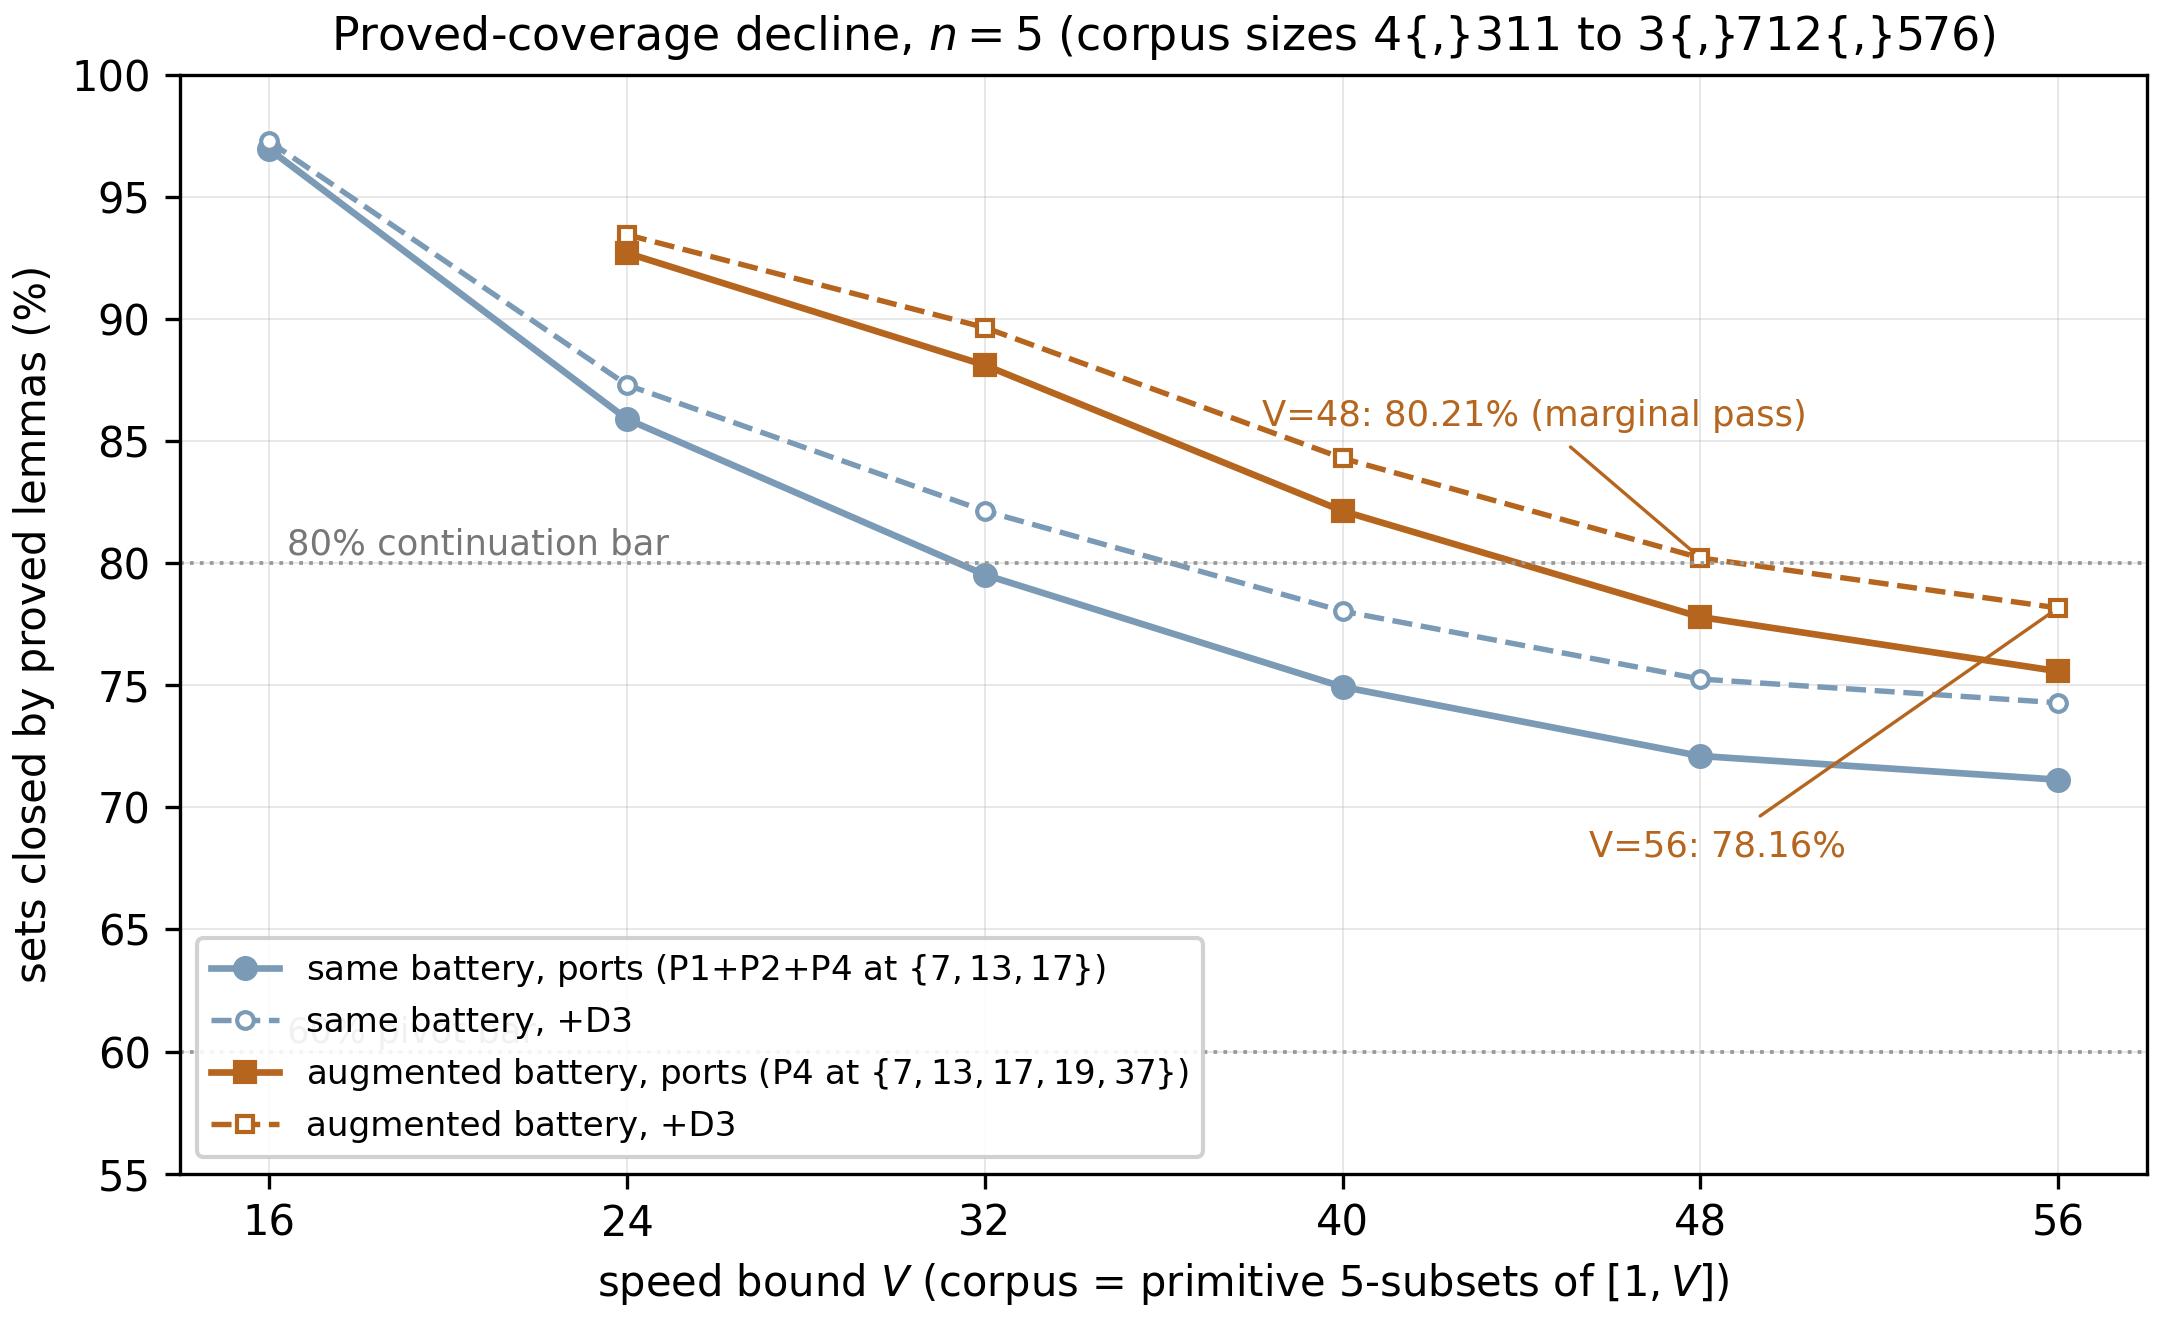
\includegraphics[max width=\textwidth, max height=0.36\textheight]
  {fig_decay.png}
\end{center}

Two framing statements, both true, must be carried together. At
\emph{matched range} ($V\le 16$, the overlap region of $4{,}311$ sets),
the reformulation performs at least as well one rung up: $96.94\%$ proved
ports at $n=5$ against $94.61\%$ at $n=4$---the strongest single datum
against the worry that the base rung closed by accident of dimension. At
\emph{growing ranges} the proved rate drops, and the drop decomposes
exactly: at $V=56$ on the same battery, the $1{,}798{,}577$ certifying
pairs that carry no proved flag split into $593{,}148$
all-invertible pairs at the then-unclassified primes $19,37$, plus
$1{,}205{,}429$ kernel-world pairs at composite moduli
($861{,}988$ at $N\le47$, $267{,}331$ at $48$--$79$, $65{,}626$ at
$80$--$95$, $10{,}484$ at $96$--$111$). After augmentation the first bucket vanishes
identifiably---the self-check ``unflagged all-invertible pair at $19$ or
$37$'' returns zero at every range---and the residual is \emph{purely}
the kernel world: mixed order signatures at composite moduli, one named
class. The classifications close a shrinking share of the verified tier
($48.4\%\to42.0\%\to28.5\%\to20.0\%\to15.1\%$ of it over $V=24\to56$) as the
incidence of $19/37$ pairs saturates; this is why the augmented curve
decays even though the rigid zone itself never grows
(\S\ref{sec:rigid}).

\subsection{The empirical pair-selection law}

The verified tier closes everything, and it does so through a striking
empirical law that deserves separate statement: \emph{at every range
measured, every single speed set has at least one certifying pair whose
$(N,\text{order signature})$ configuration is never-covering}---that is
exactly why V2 closes $100\%$. On the full $V=56$ corpus, all
$3{,}712{,}576$ sets have a certifying pair (the ground truth of
$(\mathrm{TAU}$-$_5)$ itself, now verified on every primitive $5$-set
with speeds $\le56$), the per-modulus capability and
signature-capability tables leave no set unclosed, and the hard
core---certifying pairs at \emph{capable} configurations---exists
($1{,}205{,}429$ such pairs corpus-wide, all kernel-world) but is never
load-bearing. Why a safe configuration is always available is not
understood; it is the empirical face of the pair-selection law, the
first open problem of \S\ref{sec:open}.

\subsection{Reading the decay honestly}

The reformulation's proved coverage declines as the corpus grows, and we
report the decline in both directions of honesty---what it does not
establish, and what it does. On the augmented battery, $+D_3$ coverage
runs $93.44\%\to89.64\%\to84.29\%\to80.21\%\to78.16\%$ over
$V=24\to56$; on the same battery,
$97.26\%\to87.29\%\to82.13\%\to78.03\%\to75.25\%\to74.28\%$ from
$V=16$. In residual terms the augmented series reads
$6.56\%\to10.36\%\to15.71\%\to19.79\%\to21.84\%$, with increments
$+3.80$, $+5.36$, $+4.07$, $+2.06$ points per $8$ units of $V$: roughly
linear growth with fluctuation. Five data points cannot distinguish
asymptotic deceleration from a noisy linear trend---the last increment
being the smallest is consistent with either reading---and we fit no
trend and claim none.

What the series does establish is a level fact. The $V=48$ point stood
at $80.21\%$, a marginal pass of the program's $80\%$ continuation
threshold (by $0.21$ points); the $V=56$ point falls below it at
$78.16\%$ ($1.84$ points under, with augmented ports at $75.57\%$). The
proved coverage of the present battery did not stabilize within the
tested range, and the paper's framing follows that fact. What remains
true at every range measured: open sets are zero, per-modulus
verification closes everything, every set has a certifying pair at a
never-covering configuration, and the residual is \emph{purely} the
kernel world---after the $K_{19}$/$K_{37}$ classifications, not a single
unflagged certifying pair lives at a classified prime (the self-check
``unflagged all-invertible pair at $19$ or $37$'' returns zero at every
range, both batteries). Within the tested range the reformulation is
productive; beyond it, the proved coverage of this particular battery
decays. Closing the residual requires a kernel-world structure
theorem---the analogue for composite moduli of what the class reduction
and the $K$-classifications provide for the unit world---and that theorem
is the single open mathematical problem the reformulation now has.
Whether the decay is \emph{fundamental} (an intrinsic scaling limit of
the method) or an artifact of the missing lemma family is open
problem~6 of \S\ref{sec:open}; the honest statement is that the present
data does not decide it.

\begin{remark}[the plain regime, measured correctly]\label{rem:plain}
Two notions of ``plain'' must not be conflated. A best-pair census (does
the single highest-$\tau$ pair lack polygon structure?) put the plain
share at $73\%$ at $n=5$; the battery-relevant any-pair census (does
\emph{no} pair of the set have polygon structure?) gives
$34.3\%$ at $V=24$, $36.0\%$ at $V=48$, and $35.2\%$ at $V=56$, against
$38.3\%$ at $n=4$.
The plain share does not grow with the rung on the battery basis; and
the plain regime is not monolithic---proved lemmas beyond the polygon one
close a large part of it, and every set that needs the verified tier is
plain. The difficulty at $n=5$ lives in the plain regime, but ``there''
is a third of the corpus, not three-quarters of it.
\end{remark}
